\documentclass{beamer}
\mode<presentation>
\usepackage{amsmath,amssymb,mathtools}
\usepackage{textcomp}
\usepackage{gensymb}
\usepackage{adjustbox}
\usepackage{subcaption}
\usepackage{enumitem}
\usepackage{multicol}
\usepackage{listings}
\usepackage{url}
\usepackage{graphicx} % <-- needed for images
\def\UrlBreaks{\do\/\do-}

\usetheme{Boadilla}
\usecolortheme{lily}
\setbeamertemplate{footline}{
  \leavevmode%
  \hbox{%
  \begin{beamercolorbox}[wd=\paperwidth,ht=2ex,dp=1ex,right]{author in head/foot}%
    \insertframenumber{} / \inserttotalframenumber\hspace*{2ex}
  \end{beamercolorbox}}%
  \vskip0pt%
}
\setbeamertemplate{navigation symbols}{}

\lstset{
  frame=single,
  breaklines=true,
  columns=fullflexible,
  basicstyle=\ttfamily\tiny   % tiny font so code fits
}

\numberwithin{equation}{section}

% ---- your macros ----
\providecommand{\nCr}[2]{\,^{#1}C_{#2}}
\providecommand{\nPr}[2]{\,^{#1}P_{#2}}
\providecommand{\mbf}{\mathbf}
\providecommand{\pr}[1]{\ensuremath{\Pr\left(#1\right)}}
\providecommand{\qfunc}[1]{\ensuremath{Q\left(#1\right)}}
\providecommand{\sbrak}[1]{\ensuremath{{}\left[#1\right]}}
\providecommand{\lsbrak}[1]{\ensuremath{{}\left[#1\right.}}
\providecommand{\rsbrak}[1]{\ensuremath{\left.#1\right]}}
\providecommand{\brak}[1]{\ensuremath{\left(#1\right)}}
\providecommand{\lbrak}[1]{\ensuremath{\left(#1\right.}}
\providecommand{\rbrak}[1]{\ensuremath{\left.#1\right)}}
\providecommand{\cbrak}[1]{\ensuremath{\left\{#1\right\}}}
\providecommand{\lcbrak}[1]{\ensuremath{\left\{#1\right.}}
\providecommand{\rcbrak}[1]{\ensuremath{\left.#1\right\}}}
\theoremstyle{remark}
\newtheorem{rem}{Remark}
\newcommand{\sgn}{\mathop{\mathrm{sgn}}}
\providecommand{\abs}[1]{\left\vert#1\right\vert}
\providecommand{\res}[1]{\Res\displaylimits_{#1}}
\providecommand{\norm}[1]{\lVert#1\rVert}
\providecommand{\mtx}[1]{\mathbf{#1}}
\providecommand{\mean}[1]{E\left[ #1 \right]}
\providecommand{\fourier}{\overset{\mathcal{F}}{ \rightleftharpoons}}
\providecommand{\system}{\overset{\mathcal{H}}{ \longleftrightarrow}}
\providecommand{\dec}[2]{\ensuremath{\overset{#1}{\underset{#2}{\gtrless}}}}
\newcommand{\myvec}[1]{\ensuremath{\begin{pmatrix}#1\end{pmatrix}}}
\let\vec\mathbf

\title{MatGeo Presentation - Problem 1.10.29}
\author{EE25BTECH11061 - V.Sainadh}
\date{}

\begin{document}

\frame{\titlepage}
\begin{frame}{Question}
A vector $\vec{r}$ is inclined at equal angles to the three axes. If the magnitude of $\vec{r}$ is $2\sqrt{3}$ units, find $\vec{r}$.

\end{frame}

\begin{frame}{Solution}

$\rightarrow$ A vector equally inclined to all three coordinate axes has equal components. Let the common scale be $c$. Then,
\begin{align}
	\vec{r} &= c\myvec{1\\1\\1} \\
	\norm{\vec{r}} &= |c|\sqrt{1^2+1^2+1^2} = |c|\sqrt{3}.
\end{align}
Given $\norm{\vec{r}} = 2\sqrt{3}$,
\begin{align}
	2\sqrt{3} &= |c|\sqrt{3} \\
	\implies |c| &= 2.
\end{align}
Hence,
\begin{align}
	\vec{r} = \myvec{2\\2\\2}\quad \text{or}\quad \vec{r}=\myvec{-2\\-2\\-2}.
\end{align}

\end{frame}

\begin{frame}{Plot}
\begin{figure}[h!]
   \centering
   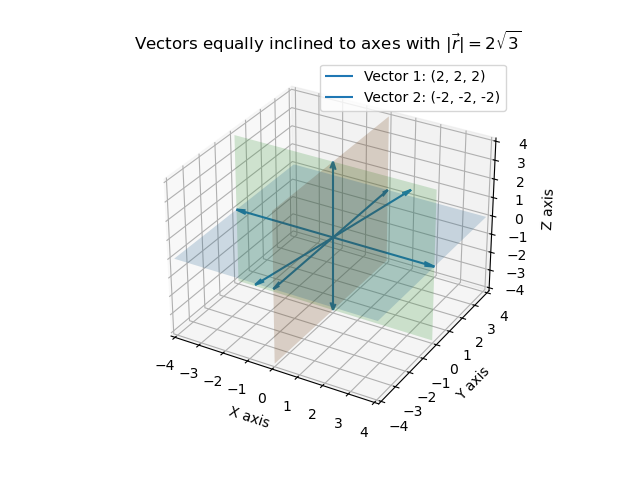
\includegraphics[width=0.8\linewidth]{figs/Figure_1.png}
   \caption{Plot of the vector $\vec{r}$}
   \label{Plot_1}
\end{figure}
\end{frame}
 % --------- CODE APPENDIX ---------
\section*{Appendix: Code}

% C program
\begin{frame}[fragile]{File: points.c}
\begin{lstlisting}[language=C]
#include <stdio.h>

int main() {
  FILE *fp;




  fp = fopen("points.dat", "w");
  fprintf(fp, "%d,%d,%d\n", 2, 2, 2);  // 1
  fprintf(fp, "%d,%d,%d\n", -2, -2, -2);   // 2
  fclose(fp);
  return 0;
  }
\end{lstlisting}
\end{frame}

% Python calling C
\begin{frame}[fragile]{File: call\_c.py}
\begin{lstlisting}[language=Python]
import subprocess

# Compile the C program
subprocess.run(["gcc", "points.c", "-o", "points"])

# Run the compiled C program
result = subprocess.run(["./points"], capture_output=True, text=True)

# Print the output from the C program
print(result.stdout)
\end{lstlisting}
\end{frame}

% Python plotting
\begin{frame}[fragile]{File: plot.py}
\begin{lstlisting}[language=Python]
import numpy as np
import matplotlib.pyplot as plt
from mpl_toolkits.mplot3d import Axes3D  # noqa: F401

# Points for |r| = 2*sqrt(3) equally inclined -> components equal (±2, ±2, ±2)
point1 = np.array([2, 2, 2], dtype=float)
point2 = np.array([-2, -2, -2], dtype=float)

# Figure and 3D axis
fig = plt.figure()
ax = fig.add_subplot(111, projection='3d')

# Vectors from origin
vector1 = point1
vector2 = point2

# Plot the two vectors
ax.quiver(0, 0, 0, vector1[0], vector1[1], vector1[2],
          label='Vector 1: (2, 2, 2)', arrow_length_ratio=0.1)
ax.quiver(0, 0, 0, vector2[0], vector2[1], vector2[2],
          label='Vector 2: (-2, -2, -2)', arrow_length_ratio=0.1)

\end{lstlisting}
\end{frame}

\begin{frame}[fragile]{File: plot.py}
\begin{lstlisting}[language=Python]

# Draw coordinate axes (both positive and negative)
scale = 4
ax.quiver(0, 0, 0,  scale, 0, 0, arrow_length_ratio=0.1)
ax.quiver(0, 0, 0, -scale, 0, 0, arrow_length_ratio=0.1)
ax.quiver(0, 0, 0, 0,  scale, 0, arrow_length_ratio=0.1)
ax.quiver(0, 0, 0, 0, -scale, 0, arrow_length_ratio=0.1)
ax.quiver(0, 0, 0, 0, 0,  scale, arrow_length_ratio=0.1)
ax.quiver(0, 0, 0, 0, 0, -scale, arrow_length_ratio=0.1)

# Plot the coordinate planes (transparent)
xx, yy = np.meshgrid(np.linspace(-scale, scale, 10),
                     np.linspace(-scale, scale, 10))
zz = np.zeros_like(xx)
ax.plot_surface(xx, yy, zz, alpha=0.2, rstride=100, cstride=100)  # XY-plane

yy, zz = np.meshgrid(np.linspace(-scale, scale, 10),
                     np.linspace(-scale, scale, 10))
xx = np.zeros_like(yy)
ax.plot_surface(xx, yy, zz, alpha=0.2, rstride=100, cstride=100)  # YZ-plane

xx, zz = np.meshgrid(np.linspace(-scale, scale, 10),
                     np.linspace(-scale, scale, 10))
yy = np.zeros_like(xx)
ax.plot_surface(xx, yy, zz, alpha=0.2, rstride=100, cstride=100)  # ZX-plane
\end{lstlisting}
\end{frame}

\begin{frame}[fragile]{File: plot.py}
\begin{lstlisting}[language=Python]

# Limits and labels
ax.set_xlim([-scale, scale])
ax.set_ylim([-scale, scale])
ax.set_zlim([-scale, scale])
ax.set_xlabel('X axis')
ax.set_ylabel('Y axis')
ax.set_zlabel('Z axis')

ax.set_title(r"Vectors equally inclined to axes with $|\vec r|=2\sqrt{3}$")
ax.legend()
plt.show()

\end{lstlisting}
\end{frame}

\end{document}